\documentclass[11pt]{article}
\usepackage{amsmath}
%\usepackage{extsizes}
\usepackage{amsmath,amssymb}
%\usepackage{omegavn,ocmrvn}
%\usepackage[utf8x]{inputenc}
\usepackage[utf8]{vietnam}

\usepackage{listings}
\lstset{language=Python}          % Set your language (you can change the language for each code-block optionally)

\usepackage{longtable}
\usepackage{answers}
\usepackage{graphicx}
\usepackage{array}
\usepackage{pifont}
\usepackage{picinpar}
\usepackage{enumerate}
\usepackage[top=3.0cm, bottom=3.5cm, left=3.5cm, right=2.5cm] {geometry}
\usepackage{hyperref}


\newtheorem{bt}{Câu}
\newcommand{\RR}{\mathbb R}
\Newassociation{sol}{Solution}{ans}
\newtheorem{ex}{Câu}
\renewcommand{\solutionstyle}[1]{\textbf{ #1}.}


\begin{document}
% \noindent
\begin{tabular*}
{\linewidth}{c>{\centering\hspace{0pt}} p{.7\textwidth}}
Trường ĐHKHTN, ĐHQGHN & {\bf Học Kỳ 1 (2019-2020)}
\tabularnewline
K62 TTƯD & {\bf Bài Tập Giải Tích Số. No 10 \\ Tính gần đúng tích phân \\ Các Quy tắc Cầu Phương Gauss}
% Exercises on pages 239, 240 Cheney/Kincaid are really nice
\tabularnewline
\rule{1in}{1pt}  \small  & \rule{2in}{1pt} %(Due date:)
\tabularnewline


%  \tabularnewline
%  &(Đề thi có 1 trang)
\end{tabular*}
%
% \Opensolutionfile{ans}[ans1]

\begin{bt}
a) Viết hàm Python dạng 
%
\begin{lstlisting}[frame=single] 
def Gauss_quad(f,a,b,nmax,eps,k):
return value, n
\end{lstlisting}
%	 
để tính gần đúng tích phân $\int_{a}^{b} f(x)dx$ trong các trường hợp cấp chính xác (kí hiệu bởi $k$) nhận các giá trị từ 1 đến 7. \\
b) Test hàm vừa viết với trường hợp $k=1$ và so sánh với quy tắc hình thang/quy tắc trung điểm khi áp dụng để tính $\int_{0}^{2} e^{-x^2}dx$.\\
c) Test hàm vừa viết với trường hợp $k=2$ và so sánh với quy tắc Simpson khi áp dụng để tính $\int_{0}^{2} e^{-x^2}dx$.
\end{bt}

\begin{bt}
Hãy áp dụng một quy tắc tính gần đúng tích phân mà các em đã viết ở trên để khẳng định hay phủ định những dự đoán sau
\begin{figure}[h!]
	\centering
	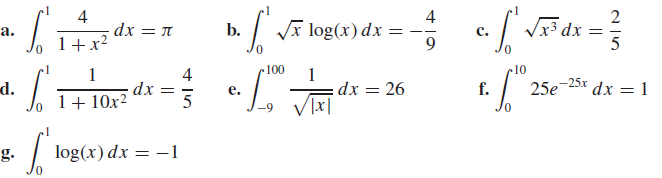
\includegraphics[width=0.9\linewidth]{1}
	\label{fig:1}
\end{figure}
\end{bt}

\begin{bt} % Exercise 5, 6 Burden Faires, p. 226
Hãy xác định các hằng số $a$, $b$, $c$, và $d$ sao cho quy tắc cầu phương sau có cấp chính xác là 3.
%
\[ \int_{-1}^{1} f(x) dx = a f(-1) + bf (1) + cf'(-1) + df'(1) \ .
 \]
%
\end{bt}

\begin{bt}
Hãy xác định các hằng số $a$, $b$, $c$, $d$, $e$ sao cho quy tắc cầu phương sau có cấp chính xác là 4.
%
\[  \int_{-1}^{1} f(x) dx = a f(-1) + bf (1) + cf(0) + d f'(-1) + e f'(1) \ .  \]
%
\end{bt}

\begin{bt}
Hãy tìm 4 hằng số $A$, $B$, $C$, $D$ sao cho quy tắc cầu phương sau có cấp chính xác lớn nhất có thể. 
%
\[  Af(-h) + B f(0) + C f(h) = hDf'(h) + \int_{-h}^{h} f(x) dx \ .
 \]%
\end{bt}

\begin{bt}
Quy tắc cầu phương
%
\[ \int_{0}^{3h} f(x) dx \approx \frac{3h}{8} \big( f (0) + 3 f (h) + 3 f (2h) + f (3h) \big) \ .
 \]%
là chính xác với mọi đa thức có bậc bé hơn hoặc bằng $n$. Tìm $n$ lớn nhất có thể.
\end{bt}

\centerline{———————————Hết——————————-}

\end{document}

\vspace{1cm}
\noindent{\bf Chú ý:} {\it Cán bộ coi thi không giải thích gì thêm}\\
\Closesolutionfile{ans}
\newpage
\begin{center}
{\LARGE{\bf ĐÁP ÁN}}
\end{center}

\begin{sol}
	\begin{figure}[h!]
		\centering
		\includegraphics[width=0.8\linewidth]{Solution1/Sol4_1.png}
		%\caption{}
		\label{fig:Sol4}
	\end{figure}
	Exercise 7: Convergence order is 3.	
\end{sol}

   
\end{document}



